%-------------------------------------------------------------------------------------------
%	Introduction to Writing
%-------------------------------------------------------------------------------------------
\section{Motivation (generalization, overparameterization)}

The text appearance and the thesis layout is sometimes determined by formal requirements. This text, for example is \NOTE{Times} using 11pt size and a slight increase in space between the text lines. There are also requirements for indenting a new paragraph sometimes.\\
As you can see, this template does not indent the new paragraph. However, you can always change this setting in the \NOTE{declarations.tex} file.\\
\ThinHRule

Some faculties require to include all references to external sources in \NOTE{footnotes}.\footnote{ This is a footnote. You can also include citations and many text formatting LaTex commands.}\footnote{ You may also explain background information on a topic, which may be interesting for further reading.}\footnote{ Footnotes also often include weblinks, for example \url{http://www.jankuester.com}}\\
\ThinHRule

You can enumerate or list some points and sketches of a topic using \NOTE{list or enumerattions}:

\begin{enumerate}
	\item Start
	\item Work
	\item Finish
\end{enumerate}


%-------------------------------------------------------------------------------------------
%	Structure of the thesis
%-------------------------------------------------------------------------------------------
\section{Brief History (language models)}

\subsection{Language Models: BERT}
Since the current template is structured into chapters, sections and subsections. This is mainly because a master thesis may easily grow up to 100 pages and in some cases even bigger. Structuring your big parts into \NOTE{chapters} makes it perfect for separating in logical units, such as:

\begin{itemize}
	\item Introduction
	\item Related Work
	\item Research Design
	\item Proceedings and Data Collection
	\item Data Analysis and Evaluation
	\item Discussion and Conclusion
\end{itemize}
\ThinHRule

The next smaller units are \NOTE{sections} which structure a chapter into it's subtopics. Using \NOTE{subsections} allows to cover these topics step by step and keep the reader on track with a mental model of all the parts of the current topic.\\
\ThinHRule

Now there are also \NOTE{subsubsections} available in LaTex. It would become very confusing when even \NOTE{including subsubsections in the table of contents (toc)}. For this reason, the toc is set to remove these subsubsections. You may alter this by taking a look into the main.tex and the declaration.tex. 
\ThinHRule

\subsubsection{\textcolor{SECTION_COL}{This Subsubsection is not listed in the Table of Contents}}

The advantage is, that your work becomes more structured along the complexity of your topic. It may occur, that topics can become very granular, which is why this is the perfect counterpart for this issue.

\subsection{Language Models: GPT-3}


%-------------------------------------------------------------------------------------------
%	Using a shorthand command
%-------------------------------------------------------------------------------------------
\section{Principles of Operation (diagrams) }

In the \NOTE{declaration.tex file}, there is a shorthand command called \NOTE{NOTE}. It is created to quickly emphasize important words and let them point out. It is declared by using the \NOTE{newcommand} tag. You may read on the web about this command, since it is very handy once you understand how to use it. You can of course create your own commands but you can also stick to this, if you want to get things done fast.


%-------------------------------------------------------------------------------------------
%	Including citations
%-------------------------------------------------------------------------------------------
\section{Formulation (math)}

Since we use the natbib environment, we need to use citep or citet as commans for our citations. This may look like the following:\\

Standard -  \citep{SkieThea2008} \citep{lombard} \citep{bendavid}\\

With page - \citep[p.123]{BernAnal2010}\\

When the authors, e.g. \citet{mayring2014} said something and you want to embed the citation in your text.

%================================================================
%
%	Basic Writing and Citing
%
%================================================================
\newpage
\section{Implementations (pre-trained models)}


%-------------------------------------------------------------------------------------------
%	Including a graphic
%-------------------------------------------------------------------------------------------
\section{Computational constraints}

Including a graphics is not that hard. Important is to wrap it as a figure, so that it will be included into the \NOTE{ list of figures}. You can also \NOTE{label} it, which allows to refer directly to this figure without the need of keeping track of it's id or name. Another handy parameter is the \NOTE{width} parameter, which allows to set the dimensions according to the current text width.

\begin{figure}[H]
\begin{center}
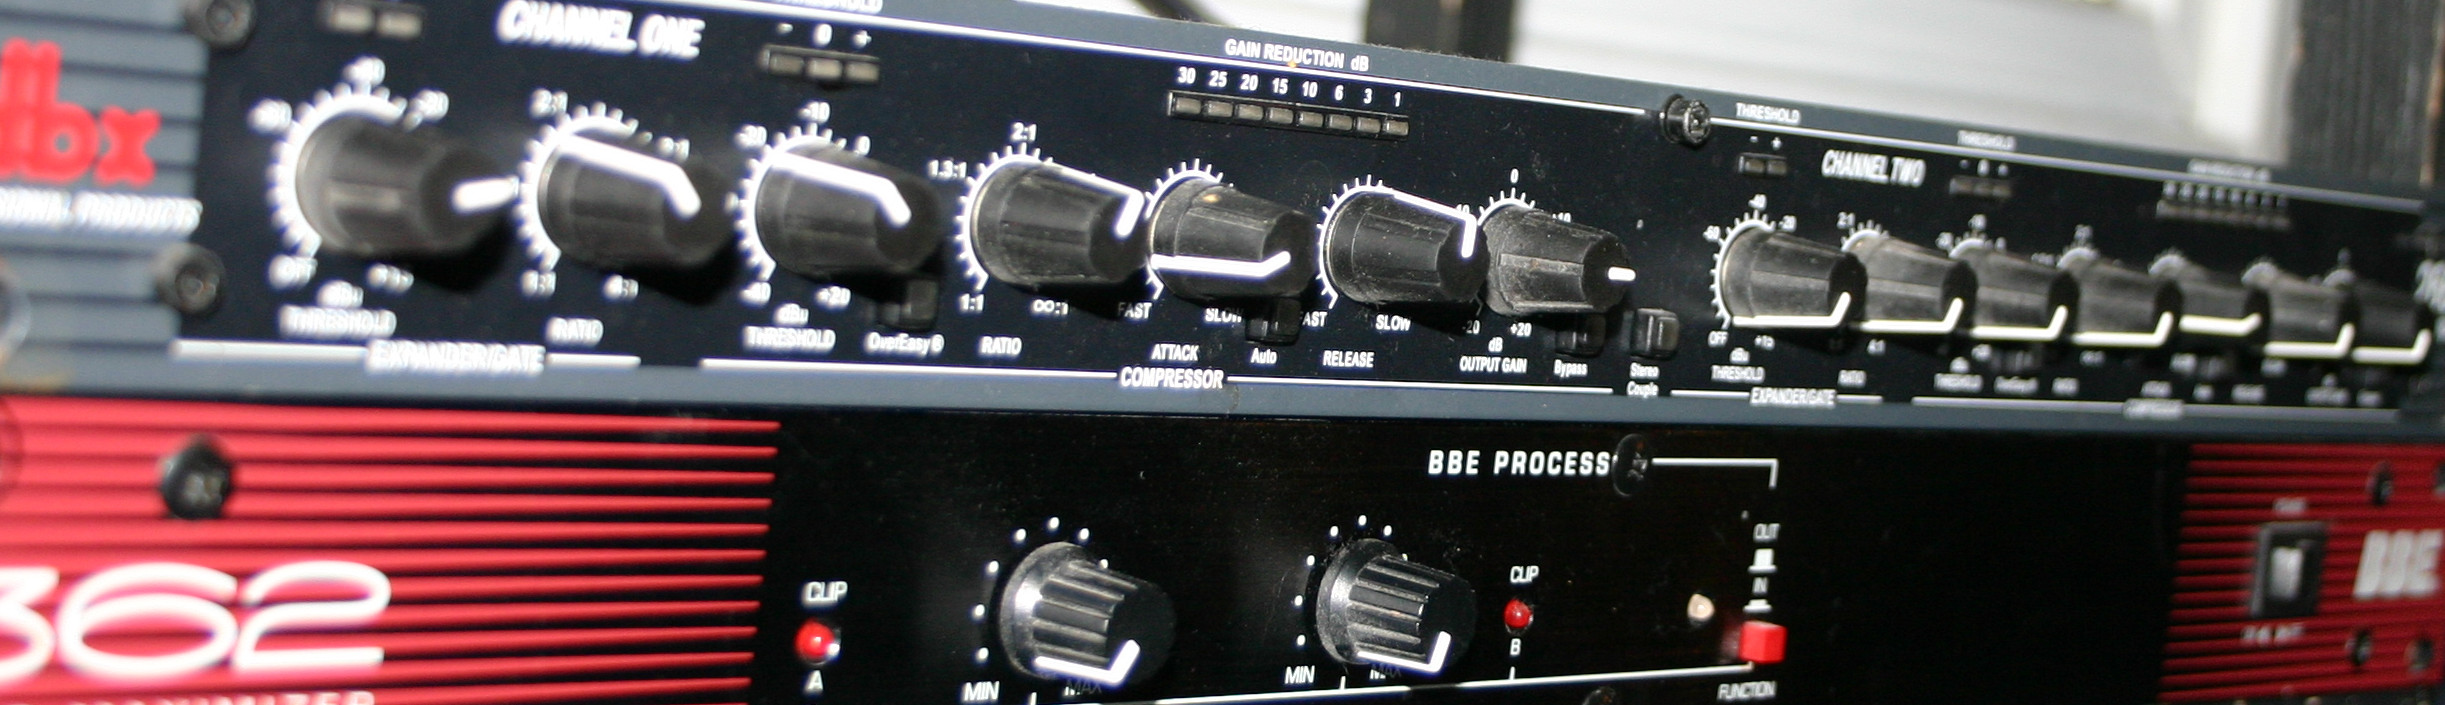
\includegraphics[width=0.8\textwidth]{media/amp.jpg}
\end{center}
\caption[Figure description for the table of content.]{This is the description of the figure. You may even include citations here, which is often important for a master thesis. For example: \citep{SkieThea2008}}
\end{figure}


%-------------------------------------------------------------------------------------------
%	Including a Table
%-------------------------------------------------------------------------------------------
\newpage
\section{Technologies used (GPU training, TACC)}

When declaring a table, you have multiple options to project complex structures. The following example uses \NOTE{multirows and multicolums} to create a multi-faceted overview of complex data. If you want the table to be listed in the \NOTE{list of tables}, you need to wrap the tabular within a table declaration.

\begin{table}[H]
\begin{tabular}{| l | l | l | l | l |}
\hline
 Category & Levels & \multicolumn{3}{c|}{Scale} \\
&&\multicolumn{3}{c|}{low \hspace*{\fill} high}\\
\hline
 \multirow{5}{*}{A} & 1. first level & low & middle & high \\ \cline{2-5}
 & 2. second level & & & \\ 
 & Subsequence & none & some &many \\
 & Extensions & none & some & all\\ \cline{2-5}
 & 3. presentation & - & text & \cellcolor{green}colored cell \\
\hline
 \multirow{5}{*}{B} & 4. fourth level &  &  &  \\ \cline{2-5}
 & graphics & low & medium & high\\ 
 & sound & mute & normal & loud \\
 & input & mouse & keyboard & gamepad\\ \cline{2-5}
 & 5. fifth leves & Low & Medium & High \\
\hline
\end{tabular}
\caption[Table description for list of tables.]{Detailed description of the table, which can also use various LaTex commands and include citations.}
\end{table}






